%%%%%%%%%%%%%%%%%%%%%%%%%%%%%%%%%%%%%%%%%
% NIWeek 2014 Poster by T. Reveyrand
% www.microwave.fr
% http://www.microwave.fr/LaTeX.html
% ---------------------------------------
% 
% Original template created by:
% Brian Amberg (baposter@brian-amberg.de)
%
% This template has been downloaded from:
% http://www.LaTeXTemplates.com
%
% License:
% CC BY-NC-SA 3.0 (http://creativecommons.org/licenses/by-nc-sa/3.0/)
%
%%%%%%%%%%%%%%%%%%%%%%%%%%%%%%%%%%%%%%%%%

%----------------------------------------------------------------------------------------
%   PACKAGES AND OTHER DOCUMENT CONFIGURATIONS
%----------------------------------------------------------------------------------------

\documentclass[a0paper,portrait]{baposter}

\usepackage[font=small,labelfont=bf]{caption} % Required for specifying captions to tables and figures
\usepackage{booktabs} % Horizontal rules in tables
\usepackage{relsize} % Used for making text smaller in some places

\usepackage{amsmath,amsfonts,amssymb,amsthm} % Math packages
\usepackage{eqparbox}

\usepackage{textcomp}

\usepackage{caption}
\usepackage{subcaption}
\usepackage{graphicx}
\usepackage{listings}
%\usepackage{verbatimbox}
%\usepackage{hyperref}

\usepackage{pgf}
\usepackage{tikz}
\usepackage[utf8]{inputenc}
\usetikzlibrary{arrows,automata}
\usetikzlibrary{positioning}


\graphicspath{{figures/}} % Directory in which figures are stored

 \definecolor{bordercol}{RGB}{40,40,40} % Border color of content boxes
 \definecolor{headercol1}{RGB}{186,215,230} % Background color for the header in the content boxes (left side)
 \definecolor{headercol2}{RGB}{120,120,120} % Background color for the header in the content boxes (right side)
 \definecolor{headerfontcol}{RGB}{0,0,0} % Text color for the header text in the content boxes
 \definecolor{boxcolor}{RGB}{210,235,250} % Background color for the content in the content boxes


\tikzset{
    state/.style={
           rectangle,
           rounded corners,
           draw=black, very thick,
           minimum height=2em,
           inner sep=2pt,
           text centered,
           },
}

\begin{document}

\setlength{\fboxsep}{0pt}

\background{ % Set the background to an image (background.pdf)
\begin{tikzpicture}[remember picture,overlay]
\draw (current page.north west)+(-2em,2em) node[anchor=north west]
{
\includegraphics[height=1.1\textheight]{background}};
\end{tikzpicture}
}

\begin{poster}{
grid=false,
columns=4,
borderColor=bordercol, % Border color of content boxes
headerColorOne=headercol1, % Background color for the header in the content boxes (left side)
headerColorTwo=headercol2, % Background color for the header in the content boxes (right side)
headerFontColor=headerfontcol, % Text color for the header text in the content boxes
boxColorOne=boxcolor, % Background color for the content in the content boxes
headershape=roundedright, % Specify the rounded corner in the content box headers
headerfont=\Large\sf\bf, % Font modifiers for the text in the content box headers
textborder=rectangle,
background=none,
headerborder=open, % Change to closed for a line under the content box headers
boxshade=plain
}
{
\includegraphics[width=3cm]{BiAtA2018.png}}
%
%----------------------------------------------------------------------------------------
%   TITLE AND AUTHOR NAME
%----------------------------------------------------------------------------------------
%
{ \bf  \huge {16s rRNA Detection by Using Neural Networks} \\  \Large \it Neural networks for secondary structure information processing} % Poster title
{\vspace{0.3em} \smaller \textbf{Semyon Grigorev$^1$}, Polina Lunina$^1$ \\  % Author names
\smaller \it $^1${Saint Petersburg State University, JetBrains, St. Petersburg, Russia } \\ % Author email addresses
\smaller  {\textbf{E-mail:} semen.grigorev@jetbrains.com}}
{
\includegraphics[width=3cm]{SPbGU_Logo.png}} % University/lab logo


%----------------------------------------------------------------------------------------
%   INTRODUCTION
%----------------------------------------------------------------------------------------
\headerbox {Motivation}{name=introduction,column=0,row=0, span=2}{

Algorithms that can efficiently and accurately identify and classify bacterial taxonomic hierarchy have become a focus in computational genetics.
The idea that secondary structure of genomic sequences is sufficient for solving the detection and classification problems lies at the heart of many tools~\cite{GrammarsRNA, PCFG, meta, LWPCFG}. 
The secondary structure can be specified in terms of formal grammars. 
The sequences obtained from the real bacteria usually contain a huge number of mutations and ``noise'' which renders precise methods impractical. 
Probabilistic grammars and covariance models (CMs) are a way to take the noise into account~\cite{EddyDurbin}.
For example, CMs are successfully used in the Infernal tool.%~\cite{Infernal}.
Neural networks is another way to deal with ``noisy'' data. 
The works~\cite{Humidor, ANN} utilize neural networks for 16s rRNA processing and demonstrate promising results. 

}

\headerbox {Results}{name=results,column=2,row=0, span=2}{
\begin{itemize} 
\item We propose the graph parsing algorithms based on different parsing techniques~\cite{GraphGLL, RelaxedRNGLR, GraphParsingGPU}.
\vspace{-0.2cm}
\item We solve some problems of existing approaches (such as cycles processing problem,~\cite{Earley}).
\vspace{-0.2cm}
\item Our solution provides an ability to use GPGPU and multi-core systems for graph parsing which can be useful for large biological data analysis.
\end{itemize}

\begin{center}
\textbf{Performance comparison of context-free querying algorithms}
\begin{tabular}{ | c | c | c | c | c |}
\hline
Graph & \#edges & \#results & GLL(ms) & GPGPU(ms) \\
\hline 
\hline
$g_{1}$     & 8688 & 141072 & 1926 & 82\\
$g_{2}$     & 14712 & 532576 & 6246 & 185\\
$g_{3}$     & 15840 & 449560 & 7014 & 127\\
\hline
\end{tabular}
\end{center}
}
    
\headerbox {Future Research}{name=future,column=2,below=results, span=2}{
\begin{itemize} 
\item Currently, we are working on long subsequences of 16s rRNA reconstruction from metagenomic assembly.
\vspace{-0.2cm}
\item We want to find new applications for context-free graph querying techniques and implement required tools.
\end{itemize}
}

\headerbox{Context-free path querying}{name=CFParsing,span=4,column=0,row=1,below=introduction}{

\begin{tikzpicture}[->,>=stealth']


\node[state,
      align=left,
      text width = 7cm] (grm) 
 {
  \textbf{Grammar}\\
 \vspace{0.3cm}  
{\ttfamily
s1: stem<s0> any
\\
a\_0\_7 : any*[2..10]
\\
s0: a\_0\_7 | a\_0\_7 stem<s0> s0
\\
any: A | U | C | G
\\
stem1<s>: A s U | G s C | U s A | C s G 
\\    
stem2<s>: stem1< stem1<s> >
\\
stem<s>:  \\
\qquad      A stem<s> U \\
\qquad    | U stem<s> A \\
\qquad    | C stem<s> G \\
\qquad    | G stem<s> C \\
\qquad    | stem1< stem2<s> >  \\
 } 
 \vspace{0.3cm}
Fixed context-free grammar describes features of secondary structure and can be tuned in order to increase result quality.
 
 };


\node[state, 
      below of=grm,
      node distance=5cm,
      align = left,
      text width = 7cm] (sqs) 
 {
 \textbf{Sequences}\\
Genom parts of fixed lengs. Current length is 512. Length is variable parameter and can be changed in order to increase quality of solution.
 };


\node[state,
      right of=grm, 
      node distance=7.5cm,
      align = left,
      text width = 6cm](parser)
{
\textbf{Parser}\\
Parser extracts features of secondary strcture.
Parsing algrithm is based on Okhotin~\cite{Okhotin} algorithm, so the grammar can be extended with cinjunctive rules for pseudocnots description.
Implementation utilizes GPGPU.
};

\node[state, 
      right of=parser,
      node distance=8cm,
      align = left,
      text width = 8.5cm] (mtrx) 
{
  \textbf{Matrices}\\
{\centering
  \fbox{
\includegraphics[width=2.5cm]{figures/mt1.png}}
  \
  \fbox{
\includegraphics[width=2.5cm]{figures/mt2.png}}
  \
  \fbox{
\includegraphics[width=2.5cm]{figures/mt3.png}}
  }
\\
Parsing result is boolean (0-1) matrix which represents secondary structure features for seqence $\omega$: cell $[i,j]$ contains 1 iff $\omega.[j,i]$ is derivale from {\ttfamily s1} and $0$ in other case. 
};

\node[state,
      below of=sqs, 
      node distance=3cm,
      align = left,
      text width = 7cm](result)
{
\textbf{Result of classification}\\
Currently we implement just binary classifier that separates 16s and non-16s sequences. 
};


\node[state,
      right of=result, 
      node distance=9cm,
      align = left,
      text width = 9.7cm](DNN)
{
\textbf{DNN}\\
\begin{minipage}[t]{5.5cm}
Dense newral network with 10 dense layers.
Trained on up to 310000 sequences of length 512: positive (16s rRNA) from NCBI database, negative (non-16s) from Green Genes database.
Current accuracy for validation set (up to 81000 sequences) is 90\%. 
\end{minipage}
\begin{minipage}[t]{4cm}
Typical building block:
\\
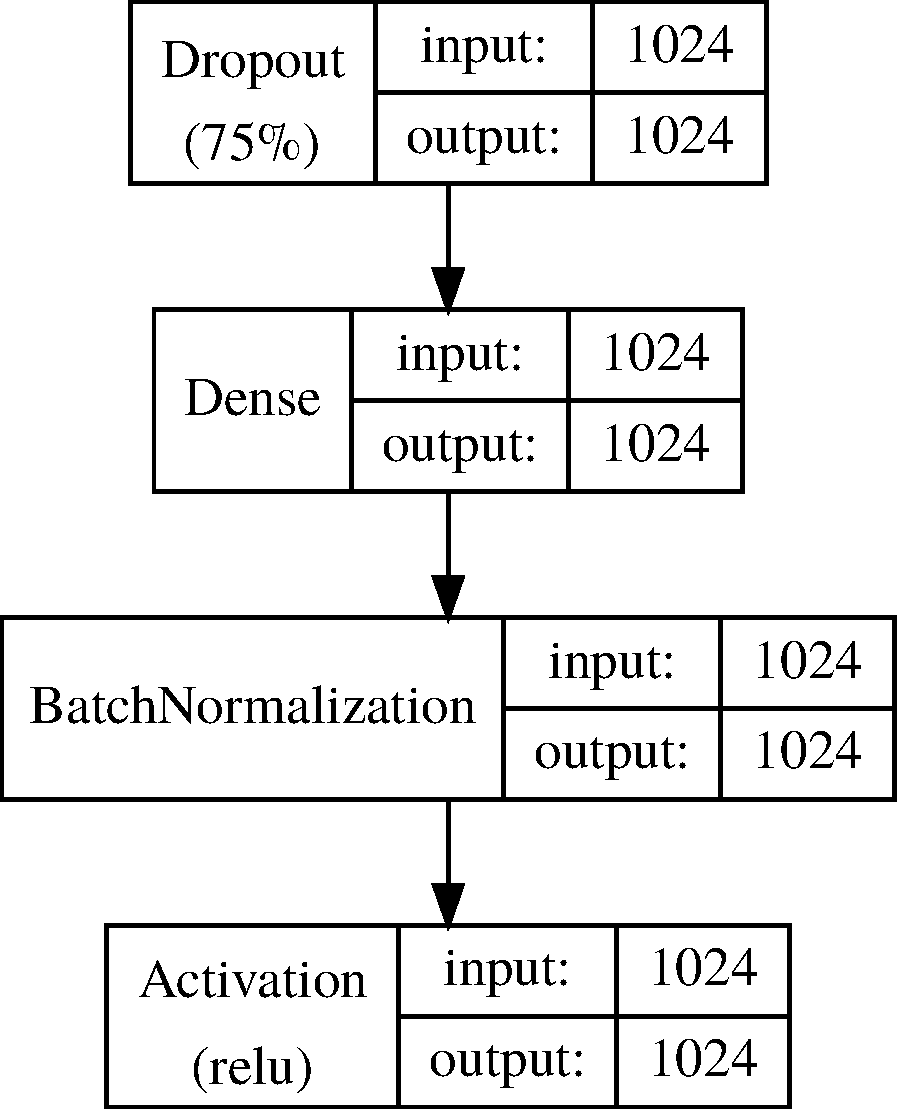
\includegraphics[width=4cm]{figures/bb.pdf}
\end{minipage}


};


\node[state,
      right of=DNN, 
      node distance=8cm,
      align = left,
      text width = 5cm](vector)
{
\textbf{Vectors}\\
Line-by-line compressed matrix representation: sequence of 32 cells is compressed to unsigned integer. Top right triangle of matrix is always empty, so can be ignored.

};


\path (grm) edge  (parser)
 (sqs) edge [bend right] (parser)
% (sqs) edge (parser)
 (parser) edge (mtrx)
 (mtrx) edge (vector)
 (vector) edge (DNN)
 (DNN) edge (result)
 ;

\end{tikzpicture}


}

\headerbox {Database querying}
{name=app1,column=0,span=2, below=CFParsing}
{ % To reduce this block to 1 column width, remove 'span=2'
One of the examples of database querying is an analysis of graphs where vertices correspond to entities and concepts such as gene or phenotype while edges represent the known relationships such as ``codes for'', ``interacts with'', etc.

Example of graph structured data~\cite{Earley} is presented below.

Querying paths with special constraints may shed light upon unknown before links between vertices, forming the basis for new hypotheses.
}


\headerbox {Metagenomic assemblies analysis}
{name=app2,column=2,span=2, below=CFParsing}
{
Metagenomic assemblies can be presented as graph structured data.
Some sequences have specific secondary structure, which can be described in terms of a context-free grammar, and this grammar can be used for searching and classification.
}


%----------------------------------------------------------------------------------------
%   REFERENCES
%----------------------------------------------------------------------------------------

\headerbox {References}{name=references,column=0,span=2,below=app1}{

\smaller % Reduce the font size in this block
\renewcommand{\section}[2]{\vskip 0.05em} % Get rid of the default "References" section title
%\nocite{*} % Insert publications even if they are not cited in the poster

\bibliographystyle{unsrt}
%\bibliographystyle{IEEEtran}
\bibliography{biblio} % Use biblio.bib as the bibliography file
}


\headerbox {Acknowledgments}{name=ack,column=2,span=1,below=app2}{
This work is supported by grant from JetBrains Research.
\vspace{0.75cm}
}
    
\headerbox {Information}{name=info,column=3,span=1,below=app2}{
All materials available on GitHub: \small{https://github.com/YaccConstructor}
\vspace{0.34cm}
}


\end{poster}

\end{document}
